\documentclass[a4paper,12pt]{scrartcl}
\usepackage{html}
\usepackage[utf8]{inputenc}
\usepackage[english]{babel}
\usepackage[T1]{fontenc}
\usepackage{graphicx}
\usepackage{xcolor}
\usepackage{url}
\usepackage{natbib}
\usepackage{hyperref}
\usepackage{ae,aecompl}
\usepackage[babel=true,final=true]{microtype}
\usepackage{subfigure}
\usepackage{amsmath}
\usepackage{amssymb}
\usepackage{gitinfo}

\newcommand*\CC{$^{13}$C}
\newcommand*\C{$^{12}$C}
\newcommand*\NN{$^{15}$N}
\newcommand*\N{$^{14}$N}
\newcommand*\OO{$^{18}$O}

\newcommand*\app{\textsc{MIA}}
\newcommand*\NTFD{\textsc{NTFD}}
\newcommand*\MD{\textsc{MetaboliteDetector}}
\newcommand*\keyctrl{\fbox{\textsc{Ctrl}}}


\title{{\large Documentation}\\\app\\{\Large Mass Isotopolome Analyzer}\\ \ \\\small\gitAbbrevHash\\ \gitCommitterIsoDate}
\author{\small Daniel Weindl\footnote{\url{mailto:sci@danielweindl.de}}}
\date{\small 2014--2016}

\hypersetup{
  colorlinks,
  urlcolor=blue,
  linkcolor=brown,
  pdftitle = {MIA - Documentation - Mass Isotopolome Analyzer},
  pdfauthor = {Daniel Weindl}
}
\setkeys{Gin}{width=5mm}
\linespread{1.2}
\setcounter{tocdepth}{3}

\begin{document}

\maketitle
 
\begin{abstract}
\textbf{\app\ is an application for non-targeted stable isotope labeling analysis. This document provides a basic overview over \app\ functionality. It is organized in two parts: a user manual and a step-by-step tutorial. The first part describes the graphical user interface (GUI), the underlying algorithms and important settings. The second part is a step-by-step tutorial that demonstrates the analysis of a sample dataset.
\newline
Additional information and the most recent version of \app\ can be found at \url{http://massisotopolomeanalyzer.lu/}.
}
\end{abstract}

\newpage\tableofcontents\newpage

\section{Introduction}

\app\ is a GUI-based software package for the non-targeted analysis of stable isotope labeling data. %TODO \citep{methodspaper}.
The detection and quantification of stable isotope labeling is based on the NTFD algorithm \citep{Hiller2010,Weindl2015a}. \app\ will detect all compounds derived from a stable isotope labeled tracer in a set of GC-MS chromatograms, visualize their corresponding mass isotopomer distributions (MIDs) and allow for further data analyses. \app\ is implemented in C++ and is based on Qt5\footnote{\url{http://qt-project.org/}}, MetaboliteDetector \cite{Hiller2009}, NTFD \cite{Hiller2010} and GraphViz\footnote{\url{http://www.graphviz.org/}} \cite{Gansner2000}. Source code and binaries for Debian-based Linux distributions as well as for Windows systems are freely available at \url{http://massisotopolomeanalyzer.lu/}.


\section{Background}
\label{sec:background}

Stable isotope labeling is widely used in metabolomics to infer metabolic fluxes or to assist chemical structure elucidation. After feeding a stable isotope labeled compound to an organism, the mass isotopomer distributions of metabolites are determined by the metabolic fluxes in the network. This is the basis for \CC\ metabolic flux analysis (\CC-MFA). To date, most mass isotopomer distribution analyses have been very targeted. \app\ offers an easy-to-use interface for determination and analysis of stable isotope labeling GC-EI-MS data in a non-targeted manner.

\app\ visualizes all detected MIDs, allows to cluster them by their similarity to find metabolically closely related compounds, offers filtering, compound identification and data export capabilities. Stable isotope labeling data from multiple datasets can be analyzed in parallel. The combined analysis of datasets from different tracers can be helpful for compound identification or pathway contextualization. The analysis of mass isotopomer distributions after feeding the same tracer under different experimental conditions can be used to globally analyze alterations in metabolic fluxes \citep{Weindl2016}.

In \citep{Weindl2016}, we show how \app\ was applied to analyze metabolism of hypoxic cancer cells and how non-targeted stable isotope labeling analysis helps provide novel biological insights.


\subsection{Non-targeted tracer fate detection (NTFD)}
\label{sec:ntfd}

The detection of stable isotope labeling in \app\ is based on the previously published NTFD algorithm \cite{Hiller2010,Hiller2013,Weindl2015a}. For NTFD, an organism is grown on standard medium and in parallel in the same medium with one or more components fully or partially replaced by their stable isotope enriched analogue. Metabolites from both cultures are extracted and subjected to GC-MS analysis. For each analyte, the mass spectra from the isotopically enriched and non-enriched sample are matched. From the difference of these mass spectra isotopically enriched fragments can be detected. For each of these fragments the mass isotopomer distribution can be calculated.

\subsection{MID-based compound networks}
\label{sec:network}

A central feature of \app\ is the visualization of labeled compound as MID-similarity-based networks. Metabolically closely related compounds show very similar MIDs. Thus, \app\ analyzes the similarity of MIDs and connects compounds with highly similar MIDs which are a sign of proximity within the metabolic network. MIDs are compared in a pair-wise manner. First, a Needleman-Wunsch-Alignment \ref{Needleman1970} is performed on the MID vectors to account for gains or losses of isotopically enriched groups. Then, the distance of these aligned vectors is calculated and the user can select a similarity threshold for which metabolites should be considered as connected \ref{sec:graph-panel}. %The highest MID similarity is observed between different silylation derivatives of the same metabolite.

The following distance measures are implemented in \app:
%\app\ uses the following distance measure:

\begin{itemize}
\item Euclidean distance \[d(p, q) = \sqrt{\sum_{i=0}^{n} (p_i - q_i)^2} \]
\item Canberra distance \[d(p, q) = \sum_{i=0}^{n} \frac{\mid p_i - q_i \mid}{\mid p_i \mid + \mid q_i \mid}\]
\item Manhattan distance \[d(p, q) = \sum_{i=0}^{n} \mid p_i - q_i \mid \]
\end{itemize}

where $p$ and $q$ are the aligned MID vectors in $\mathbb{R}^n$ of the first and second analyte respectively. The MID distances can be normalized to the length of the MID vectors.

\subsection{MID variation filtering}
\label{sec:variation}

When comparing stable isotope labeling after feeding the same tracer under different experimental conditions, it is interesting to detect changes in mass isotopomer distributions since they are indicative of changes in metabolic fluxes \cite{Weindl2015b,Weindl2016}. To detect compounds with varying labeling patterns, \app\ allows to filter the results by variation in their MIDs. Therefor the maximum standard deviation in relative mass isotopomer abundance is determined for every compound and the user can hide compounds with low variation score (\ref{sec:graph-panel}).
\[\text{variation score} = \max \sigma \quad \mid \quad \sigma_i = \sqrt{\frac{1}{n} \cdot \sum_{j=0}^{n} (\overline{p}_i - p_{i,j})^2} \] where $p_{i,j}$ is the relative abundance of the M + $j$ isotopologue of the given compound in the $i$-th dataset. The MIDs of unlabeled compounds are not considered.\footnote{Compounds which are only labeled under specific conditions are also of interest. However, they need to be checked for false positives.}

\section{User manual}

\subsection{Installation}

Installation packages for \app\ can be downloaded from \url{http://massisotopolomeanalyzer.lu/} in the .deb or .exe format. Alternatively, you can download a plain archive with the binaries.

\subsubsection{Linux}

Open a terminal and change to the directory containing the downloaded file. Then type the following in the command line:

% \texttt{sudo rpm -i filename} for rpm based systems

\texttt{sudo dpkg-i filename.deb} for Debian based systems

where filename is the name of the deb %or rpm
installation package (e.g \texttt{mia-1.0-Linux.deb}).

\subsubsection{Windows}

Unpack the \app-Windows archive and run \texttt{mia-gui.exe}

\subsection{Graphical user interface (GUI)}
\label{sec:gui}

The graphical user interface is organized in one mainwindow containing three subwindows which are explained below. Several application settings can be changed in the configuration dialog (\ref{sec:settings}).

\subsubsection{Main window}

\label{sec:mainwindow}

\begin{figure}[htb]
 \centering
 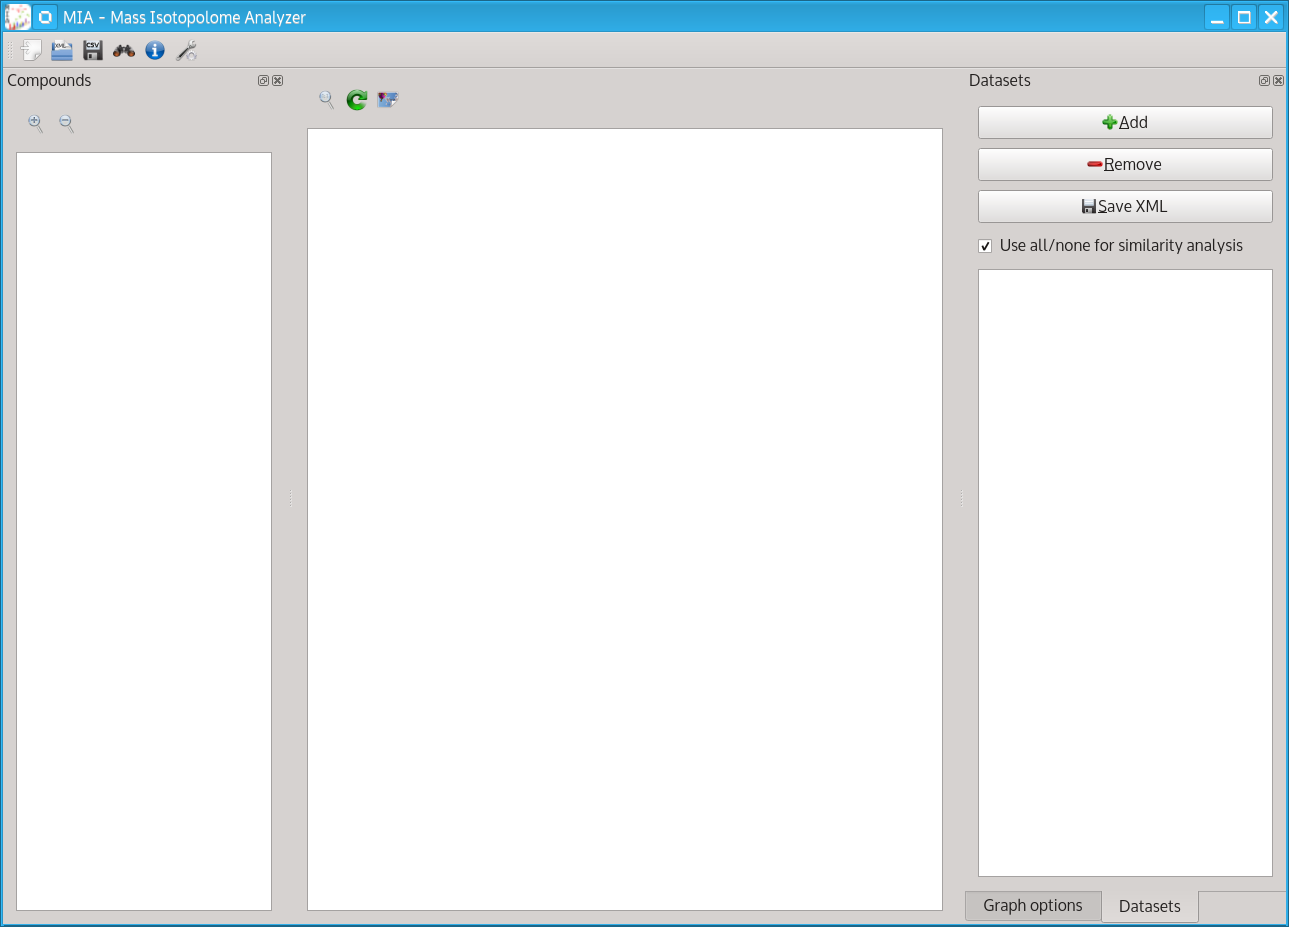
\includegraphics[width=0.8\linewidth]{./gfx/ss_mainwindow_empty.png}
 \caption{\app\ Main window with the graph view in the center, the main toolbar at the top (\ref{sec:maintoolbar}), the compound panel (\ref{sec:compound-panel}) on the left and the experiments (\ref{sec:dataset-panel}) and graph panel (\ref{sec:graph-panel}) on the right.}
 \label{fig:mainwindow}
\end{figure}

The mainwindow toolbar (Fig.~\ref{fig:mainwindow}) provides the following functionality:

\paragraph{Main toolbar}
\label{sec:maintoolbar}

\begin{description}
% \item[
\includegraphics{gfx/ico_open.png} Open binary data]
% Load dataset from \app\ binary data file.

\item[
\includegraphics{../gui/icons/document-import.png} Import data]
Opens the data import panel (\ref{sec:data-import}) to import GC-MS data from the netCDF format or perform peak detection on chromatograms in the MetaboliteDetector \citep{Hiller2009} format.

\item[
\includegraphics{../gui/icons/document-open-xml.png} Open XML]
Load dataset from \app\ XML configuration file.

\item[
\includegraphics{gfx/ico_save.png} Save binary data]
Save current dataset to \app\ binary data file.

% \item[
\includegraphics{../gui/icons/document-save-hdf5.png} Export results to HDF5]
% Save MID distance matrix (\ref{sec:network}) in HDF5 format\cite{hdf5}.

\item[
\includegraphics{../gui/icons/document-save-csv.png} Export MIDs to CSV]
Save MIDs of all detected labeled fragments to comma separated values (CSV) file. The exported data can be opened with common spreadsheet programs like OpenOffice Calc or Microsoft Excel.

\item[
\includegraphics{gfx/edit-find.png} Library search]
Try to identify the detected compounds (see~\ref{sec:compound-panel}) based on a \MD\ reference library. Matching is performed on spectrum similarity and retention index available (\ref{sec:identification}). % TODO dialog, multiple libraries in the order of selection

\item[
\includegraphics{gfx/ico_about.png} About]
Show \app\ version information.

\item[
\includegraphics{gfx/ico_settings.png} Application settings]
Shows the settings dialog (see~\ref{sec:settings}).

% \item[
\includegraphics{gfx/ico_library.png} Generate \MD\ library]
% Generate a library with the spectra detected labelled compounds for use in \MD.
\end{description}

\subsubsection{Graph view}

\label{sec:graph-view}

The central component of the \app\ GUI is the graph view. Here you can find a lot of information on all labelled compounds detected in the active datasets. 
The layout and the compounds shown depend on the settings in the experiment panel (\ref{sec:dataset-panel}), the graph panel (\ref{sec:graph-panel}) and the settings dialog (\ref{sec:settings}).

\begin{figure}[htb]
 \centering
 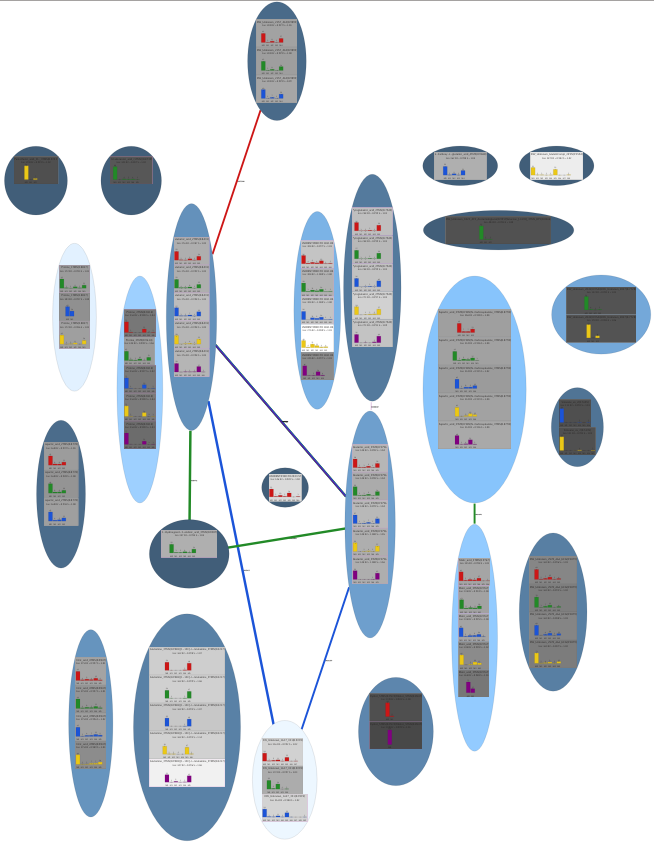
\includegraphics[width=0.7\linewidth]{./gfx/ss_mainwindow_graphview.png}
 \caption{The graph view.}
 \label{fig:graph-view}
\end{figure}

\label{sec:node}
For every compound the MID of the selected labeled fragment (usually the largest) is shown for each active dataset (\ref{fig:compound-node}). The background color of the ellipse reflects the variation in relative mass isotopomer abundance, ranging from dark blue (low) to high (white). The MID plots for each dataset set show the relative mass isotopomer abundances as bars with 95\% confidence intervals and numbers, the compound name (after identification - see \ref{sec:identification}), the selected $m/z$, and some quality measures. The background color reflects the amount of isotopic enrichment ($1-M_0$)\footnote{The value of $1-M_0$ is used, since the actual isotopic enrichment $1/n \cdot \sum i\cdot M_i$ cannot be determined because the number of possibly labeled atoms $n$ is not known before compound identification and knowledge on fragmentation.}, ranging from dark gray (unlabeled) to very light gray (fully labeled). As quality measures, there are the coefficient of determination $R^2$ (``R2'') and the sum of absolute mass isotopomer abundances (``S''). Both these values should ideally be equal to 1 \citep{Weindl2015a}. Thresholds for both can be defined in the label detection parameters in the experiment wizard (\ref{sec:experiment-wizard}).

%TODO coloring

\begin{figure}[htb]
 \centering
 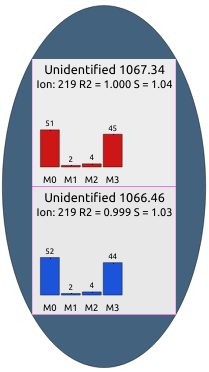
\includegraphics[width=0.2\linewidth]{./gfx/ss_node.png}
 \caption{A node in the graph view showing mass isotopomer distributions and some quality measures.}
 %TODO tool tip screenshot
 \label{fig:compound-node}
\end{figure}

Double click the oval to pop-up the detailed compound view (\ref{sec:compound-details}) (you can open multiple windows) or hold the mouse for a tooltip with additional information.

%TODO molecular ion, 
% TODO Additional information if the graph feature is used line width, distance, ... color 

\paragraph{Navigation}
You can zoom in and out of the graph view by holding \keyctrl\ and using the mouse wheel. You can reset the zoom by clicking 
\includegraphics{gfx/ico_zoom-original.png} in the toolbar. To navigate through the graph view, you can use the scroll bars, or the mouse wheel or scroll keys, or move the mouse while holding the middle button.

\paragraph{Toolbar actions}
\begin{description}
\item[
\includegraphics{gfx/ico_zoom-original.png} Reset zoom]
Reset zoom to fit all plots into the view.

% \item[\includegraphics{gfx/.png} Refresh]
% Repaint the graph.

\item[
\includegraphics{gfx/ico_export-image.png} Export image]
Export the current graph as scalable vector graphics (SVG). The exported file can easily be edited with most vector graphics applications like e.g. Inkscape\footnote{\url{http://www.inkscape.org/}}. Individual plots can easily be copied and modified from there to include them in other documents or presentations.
\end{description}

\subsubsection{Compound detail view}
\label{sec:compound-details}

Double-clicking a node in the graph pops up the compound details view (Fig.~\ref{fig:compound-details}). There, you can find MID plots for all isotopically enriched fragments in all active datasets and some additional information.

\begin{figure}[htb]
 \centering
 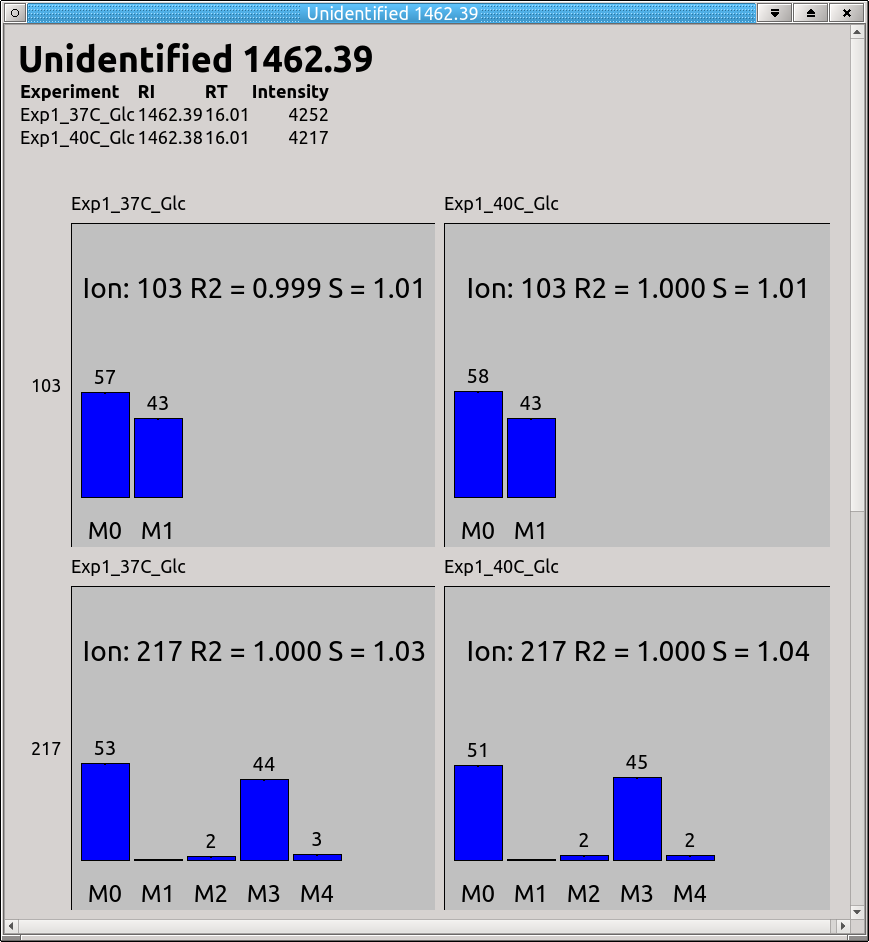
\includegraphics[width=0.6\linewidth]{./gfx/ss_compound_details.png}
 \caption{The compound details window showing MID plots for all isotopically enriched fragments in all active datasets and some additional information.}
 \label{fig:compound-details}
\end{figure}

Below the name, you can find the datasets in which the given compound was found to show isotopic enrichment along with its retention time (RT) and retention index (RI). The array of plots shows the MIDs of all labeled fragments (in rows) in all active datasets (in columns). The plot details are explained above (\ref{sec:node}). Double-clicking a plot will copy the corresponding mass MID to the system clipboard.

\subsubsection{Compound panel}

\label{sec:compound-panel}

The compound panel (Fig.~\ref{fig:compound-panel}) is displayed in left part of the \app\ main window. It lists all compounds which show isotopic enrichment in any of the currently active datasets. MIDs of all labeled fragments can be viewed after clicking the expand icon in the tree view. Click on the compound name to center the graph view (\ref{fig:graph-view}) on this compound.

\begin{figure}[htb]
 \centering
 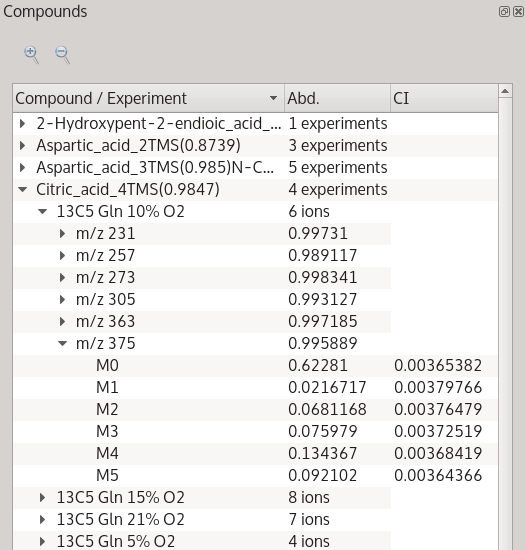
\includegraphics[width=0.4\linewidth]{./gfx/ss_compound_panel.png}
 \caption{The compound panel.}
 \label{fig:compound-panel}
\end{figure}

The toolbar provides the following functionality:

\begin{description}

\item[
\includegraphics{gfx/ico_zoom-in.png} Expand]
 Expand the tree view and see the following information:
\begin{center}
\fbox{
\begin{tabular}{lllll|l|l}
$+$ & \multicolumn{4}{l|}{Compound name} & \# datasets & \\
  & $\llcorner$ & \multicolumn{3}{l|}{Dataset}  & \# ions  &\\
  & & $\llcorner$ & \multicolumn{2}{l|}{Labelled fragment $m/z$}& $R^2$ & \\
  & & & $\llcorner$ & Mass isotopomer & abundance & 95\% confidence interval\\
\end{tabular}
}
\end{center}
This information can be exported as CSV from the main toolbar (
\includegraphics{../gui/icons/document-save-csv.png} - \ref{sec:maintoolbar}).

 \item[
\includegraphics{gfx/ico_zoom-out.png} Collapse]
 Collapse the tree view to only show the list of labelled compounds. 
\end{description}

\subsubsection{Dataset panel}

\label{sec:dataset-panel}

This panel shows the currently loaded datasets and allows you to add or remove new data sets (Fig.~\ref{fig:experiment-panel}). The table shows the name of your dataset  and the number of isotopically enriched compounds and non-enriched compounds. With the checkbox in the first column you can select which datasets should be used for the network generation (\ref{sec:network} and \ref{sec:graph-panel}).

To add a new dataset hit ``Add'' and follow the experiment wizard (\ref{sec:experiment-wizard}). To remove a dataset, select it in the table and hit ``Remove''. The settings for label detection and compound identification can be edited by double clicking the corresponding dataset in the table (\ref{sec:experiment-wizard}).


\begin{figure}[htb]
 \centering
 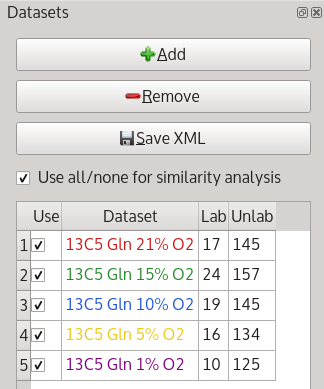
\includegraphics[width=0.4\linewidth]{./gfx/ss_experiment_panel.png}
 \caption{List of currently active datasets.}
 \label{fig:experiment-panel}
\end{figure}

\subsubsection{Add and Edit datasets}
\label{sec:experiment-wizard}

New datasets are added or existing datasets are modified via the experiment wizard which can be opened by clicking ``Add'' or double clicking a dataset in the experiment panel (\ref{sec:dataset-panel}). The first page asks for a name and the data files for the dataset (Fig.~\ref{fig:experiment_files}).


\begin{figure}[htb]
 \centering
 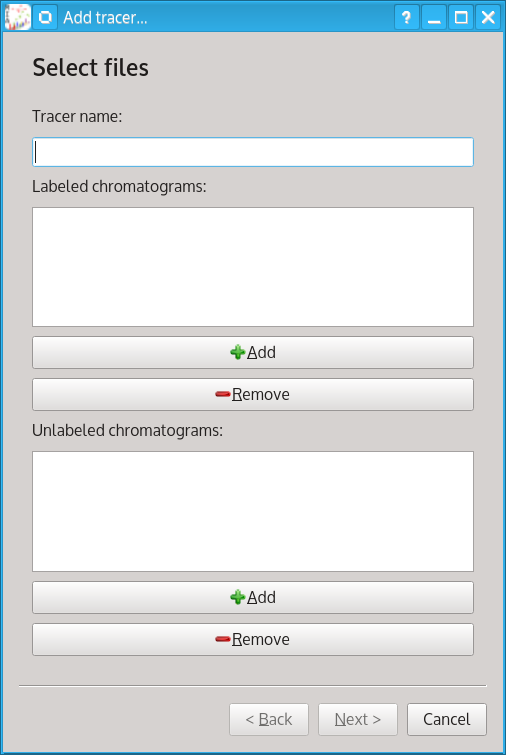
\includegraphics[width=0.4\textwidth]{./gfx/ss_experiment_files.png}
 \label{fig:experiment_files}
 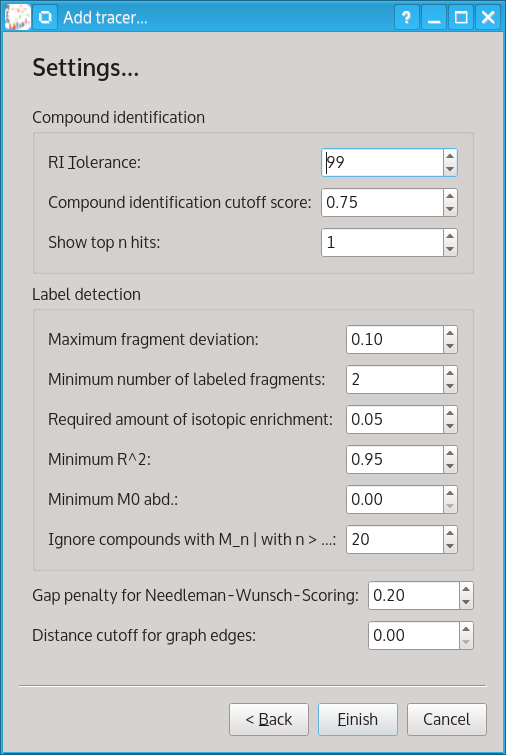
\includegraphics[width=0.4\textwidth]{./gfx/ss_experiment_settings.png}
 \caption{The experiment wizard page for file selection and for label detection and compound identification.}
 \label{fig:experiment_settings}
\end{figure}

\begin{description}
 \item[Name] 
 An arbitrary name for the dataset.
 \item[(Un)Labeled chromatograms]
 Data files from the measurements of the (un)labelled metabolite extract (\ref{sec:ntfd}). If multiple data files are added here, confidence intervals can be calculated for the MIDs \cite{Hiller2010}. Data from multiple independent experiments should added as separate dataset, not as multiple chromatograms for the same dataset. 
\end{description}

On the second wizard page, a number of parameters can be set for the detection of isotopic enrichment, compound identification, and a few more things:\footnote{The default settings are a good starting point for most applications, but should be adjusted for optimal results.}

\paragraph[Detection of isotopic enrichment]{Detection of isotopic enrichment:\footnote{See also \NTFD\ documentation available at \url{http://ntfd.mit.edu/} and \cite{Weindl2015a}}}

\begin{description}
 \item[Maximum fragment deviation]
 The maximum allowed value for $1 - \sum \mid M_i \mid$ (important quality filter).
 
 \item[Minimum number of labeled fragments]
 Compounds with a number of labeled fragments lower than this number will be ignored.
 
 \item[Required amount of isotopic enrichment]
 Minimum value for $1 - M_0$.
 
 \item[Minimum R\^ 2]
 Minimum allowed coefficient of determination $R^2$ for each fragment. 
 
 \item[Minimum M0 abd.]
 The minimum relative abundance of the M+0 mass isotopomer.
 
 \item[Ignore compounds with M\_n $\mid$ with n > ...]
 The upper limit for MID size.
\end{description}

\paragraph{Compound identification:}
\begin{description}
 \item[RI tolerance]
 Changes the influence of the retention index (RI) on the compound identification score.
 
 \item[Matching score cutoff]
 Defines the threshold for the spectrum matching score above which a library compound is considered as a hit.
 
 \item[Show top $n$ hits]
 Defines how many compound identification hits should be kept as the label.
\end{description}

\paragraph{Others:}
\begin{description}
 \item[Gap penalty for Needleman-Wunsch-Scoring]
 Gap penalty used for the Needleman-Wunsch alignment of MIDs for the distance calculation (\ref{sec:network}).

 \item[Distance cutoff graph edges]
 Distance cut-off for MID similarity analysis (\ref{sec:network}). This value should not be modified here, but in the graph settings panel (\ref{sec:graph-panel}).
\end{description}

\subsubsection{Save XML}

To avoid repeatedly selecting the data files and adjusting the settings you can save the settings in an XML file which can later be reloaded by clicking 
\includegraphics{../gui/icons/document-open-xml.png} ``Open XML'' in the main toolbar.

Note: \app\ saves absolute paths to the data in the .xml files. If the data was moved, the paths can be adjusted in the .xml file using a standard text editor.

\subsubsection{Graph panel}

\label{sec:graph-panel}

The graph panel (Fig.~\ref{fig:graph-panel}) contains the settings for the generation of the compound networks (\ref{sec:network}).

\begin{figure}[htbp]
 \centering
 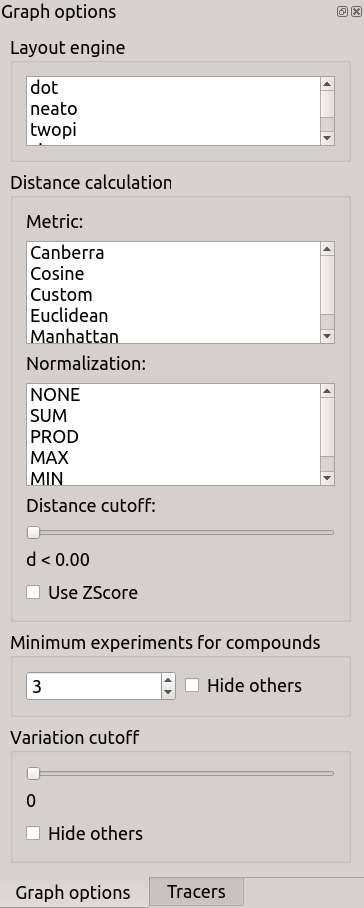
\includegraphics[width=0.3\linewidth]{./gfx/ss_graph_panel.png}
 \caption{Graph panel to setup the compound network to connect compounds by MID similarity (\ref{sec:network}).}
 \label{fig:graph-panel}
\end{figure}

\begin{description}
 \item[Layout engine]
 The \textsc{GraphViz} engine to layout the graph. See \textsc{GraphViz} documentation for more information. ``dot'' is the default and recommended.
 
 \item[Distance metric]
 Metric used to calculate MID distance (\ref{sec:network}).
 
 \item[Distance normalization]
 Optional normalization factor for MID distances.
 %TODO norm
 
 \item[Distance cutoff]
 MIDs with distances below the given threshold are considered as connected in the compound graph.
 
%  \item[Use z-score]
% z-score
 
 \item[Minimum experiments]
 The minimum number of datasets in which the compound has to be detected as isotopically enriched to be considered for the compound graph. Select ``Hide others'' to hide all nodes detected as labeled in a lower number of datasets.
 
 \item[Variation cutoff]
 The minimum value for the variation score (\ref{sec:variation}) for each node to be considered for the compound graph. Select ``Hide others'' to hide all nodes with a lower variation score.
\end{description}

\subsubsection{Compound identification}
\label{sec:identification}
%TODO id , MD, RI, lib selection, multiple

The detected isotopically enriched compound can be matched against a mass spectrum library for compound identification by selecting 
\includegraphics{gfx/edit-find.png} ``Library search'' from the main toolbar. Currently, only MetaboliteDetector \citep{Hiller2009} libraries are supported.\footnote{If you do not have a compound library in the MetaboliteDetector format available already, the \textit{Golm Metabolome Database} (GMD) \cite{Hummel2013} provides a good start. Download their mass spectral database in the MSL format from \url{http://gmd.mpimp-golm.mpg.de/download/} and create a library file from it using MetaboliteDetector (\url{http://metabolitedetector.tu-bs.de/}) by selecting \textit{File} $\rightarrow$ \textit{Import} $\rightarrow$ \textit{Import MSL library}. The resulting .lbr file can be used with \app.}

\app\ uses a spectrum and RI / RT based algorithm for spectrum matching. The RI tolerance and identification score cutoff can be defined in the experiment wizard (\ref{sec:experiment-wizard}).


\subsubsection{Settings}

\label{sec:settings}

The settings dialog (Fig.~\ref{fig:settings_paths}) can be opened by clicking 
\includegraphics{gfx/ico_settings.png} in the main toolbar (\ref{sec:maintoolbar}).
More graph options and certain default paths can be set here (Fig.~\ref{fig:settings_paths}).

\begin{figure}[htb]
 \centering
 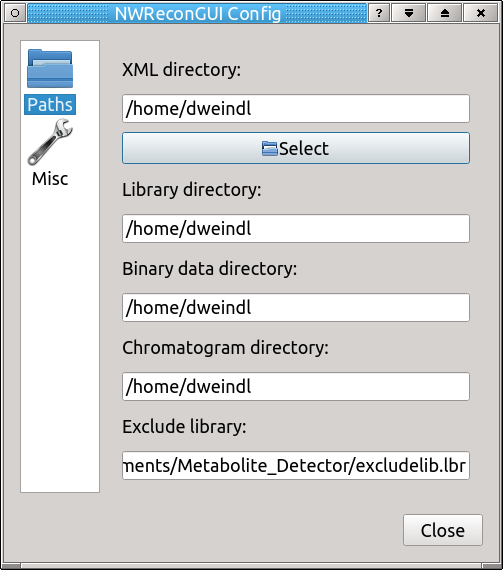
\includegraphics[width=0.4\linewidth]{./gfx/ss_settings_paths.png}
 \label{fig:settings_paths}
 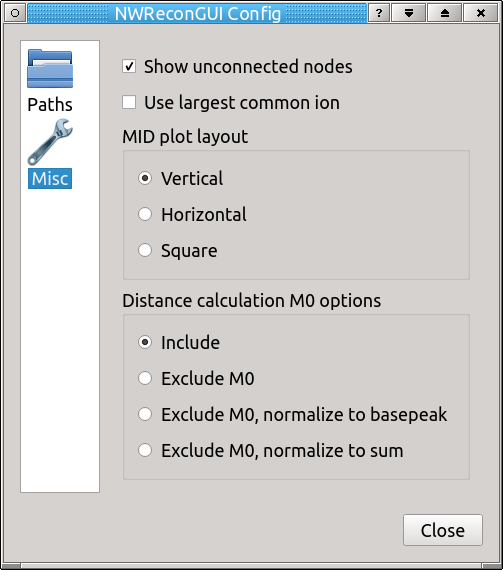
\includegraphics[width=0.4\linewidth]{./gfx/ss_settings_misc.png}
 \caption{The configuration page for paths and miscellaneous settings.}
 \label{fig:settings_misc}
\end{figure}

\begin{description}
 \item[Show unconnected nodes]
 Toggle whether nodes which are not connected to any others nodes should be shown or not (see also \ref{sec:graph-panel} and \ref{sec:network}).
 
 \item[Use largest common ion]
 If a compound was detected in multiple datasets, the heaviest labeled fragment common to all datasets can be used in the plot and for distance calculation, or the heaviest fragment for each dataset independently.
 
 \item[MID plot layout]
 MID plots for a compound labeled in multiple experiments can be laid out vertically, horizontally or in a quadratic grid.
 
 \item[Distance calculation]
 Defines on which data the MID distance calculation is performed. The full MID vector can be used (``Include'') or the M+0 can be omitted (``Exclude M0''). If M+0 is omitted, the remaining vector can be divided by the highest value ("normalize to basepeak``) or the sum (''normalize to sum``).
 
\end{description}

\subsubsection{Data export}

\label{sec:data-export}

An important feature of \app\ are its data export capabilities.

The following data can be exported:
\begin{description}
 \item[MIDs of all compounds detected as isotopically enriched]
 By selecting 
\includegraphics{../gui/icons/document-save-csv.png} ''Export MIDs to CSV`` from the main toolbar

 \item[MID plots of all compounds and the MID similarity-based network]
  By selecting 
\includegraphics{gfx/ico_export-image.png} ''Export image`` in the graph view toolbar (\ref{sec:graph-view})

 \item[MID plots for all fragments of each compound]
  By selecting 
\includegraphics{gfx/ico_export-image.png} ''Export image`` in the Compound detail view (\ref{sec:compound-details})

 \item[The settings used for the analysis]
  By selecting ''Save XML`` in the dataset panel (\ref{sec:dataset-panel})

\end{description}

% TODO hdf

\subsubsection{Data import}

\label{sec:data-import}

\app\ requires data in the MetaboliteDetector \citep{Hiller2009} format. GC-MS data can be imported from the netCDF format via the data import dialog (Fig.~\ref{fig:data-import}) which can be accessed via 
\includegraphics{../gui/icons/document-import.png} ''Import data`` in the main toolbar. This dialog can also be used to re-perform peak picking and spectrum deconvolution on existing MetaboliteDetector data.

Note: For best control over deconvolution, these steps should be performed in MetaboliteDetector where they can be inspected immediately. Low quality spectra should already be filtered at this stage to increase specificity and speed of the detection of isotopic enrichment.

\begin{figure}[htb]
 \centering
 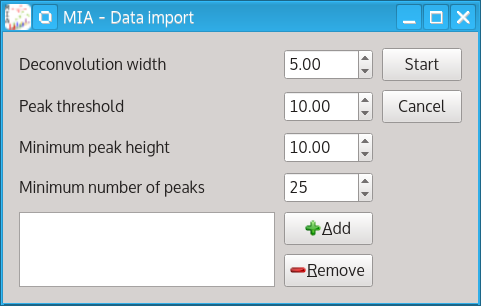
\includegraphics[width=0.4\linewidth]{./gfx/ss_data_import.png}
  \caption{Data import window}
 \label{fig:data-import}
\end{figure}

\clearpage

%\section{FAQ}
%TODO FAQ
%\clearpage

\section{Step-by-step tutorial}

On the \app\ website, there is a sample data set available for download. In the following, we will demonstrate the first steps in \app\ to explore this stable isotope labeling data.

The sample data set contains GC-MS measurements of trimethylsilylated metabolite extracts from A549 cells incubated under 21\% or 1\% oxygen atmosphere (''N`` / ''H``)in the presence of [U-$^{13}$C]glucose (''U13CGlc``), [U-$^{13}$C]glutamine (''U13CGln``) or only unlabeled substrates (''``). The data is supplied ready-to-use in the MetaboliteDetector format (.bin/.idx/.cmp).

\subsection{Start program and load data}

Download and unpack the sample data and run \app. For a quick start, the file \texttt{sampleData.xml} contains all parameters for the given data sets and can be loaded by selecting 
\includegraphics{../gui/icons/document-open-xml.png} ''Open XML`` from the main toolbar.

Note: \texttt{sampleData.xml} must be located in same folder as the data files.

After selecting the .xml file, compound detection will start automatically. Depending on your system, this might take up to a few minutes. Once, compound detection is finished, you will see all compounds which were detected as isotopically enriched (Fig.~\ref{fig:tutorial-dataloaded}).

\begin{figure}[htbp]
 \centering
 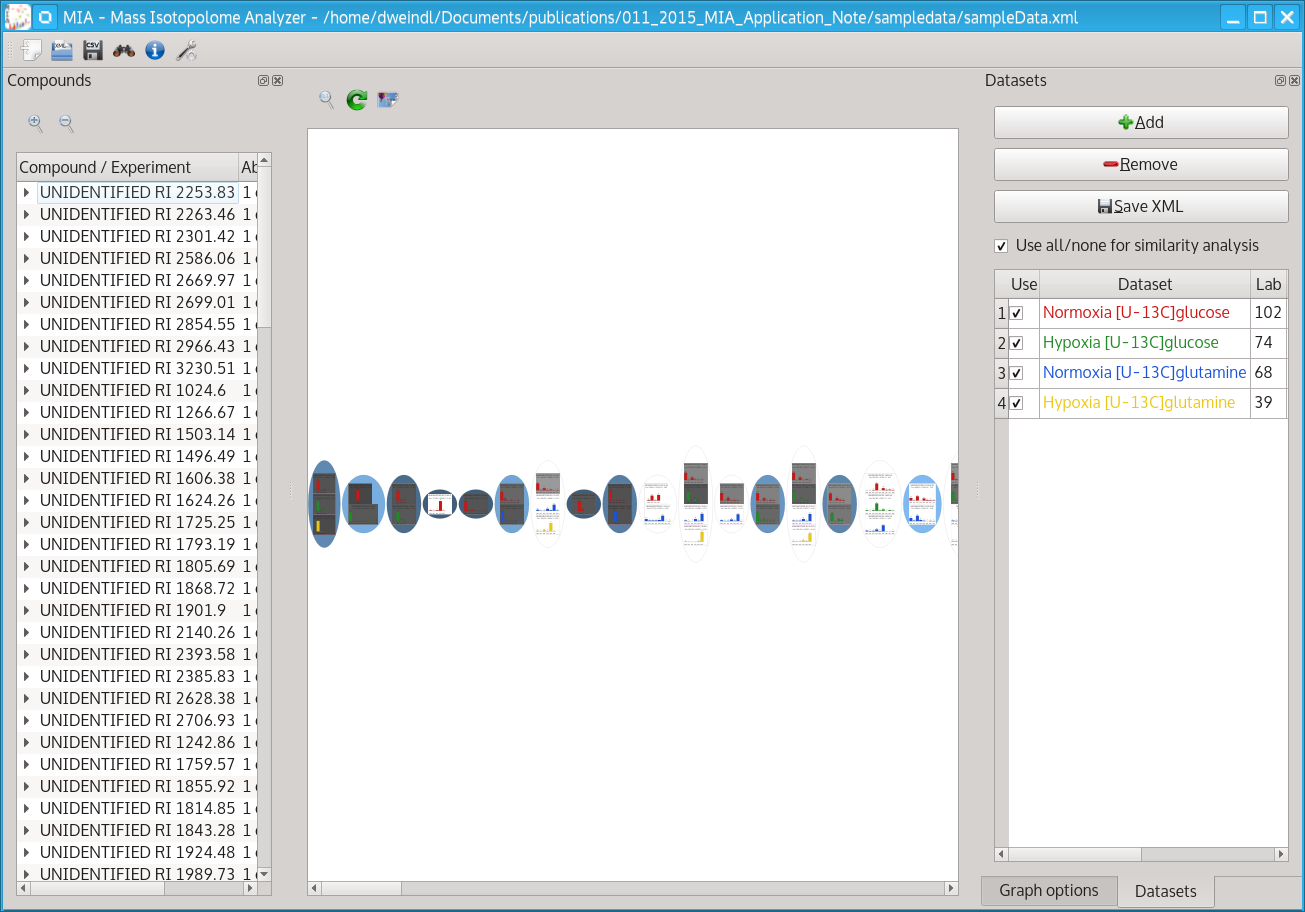
\includegraphics[width=0.8\textwidth]{./gfx/ss_tutorial_dataloaded.png}
 \caption{\app\ after loading the sample dataset.}
 \label{fig:tutorial-dataloaded}
\end{figure}

%Although \app\ can import data from the netCDF format it is highly recommended to perform peak detection and deconvolution in \href{http://metabolitedetector.tu-bs.de/}{\MD} \citep{Hiller2009}


\subsection{Inspecting the results}

In the dataset panel, you can see the different experimental conditions and how many compounds were detected as isotopically enriched. In the center, you can see every detected enriched compound as an ellipse with plotted MIDs for each experimental condition with the same color coding as on the list on the right (see \ref{sec:node}). The compound panel on the left shows a list of all compounds which were detected in any of the datasets. For now, these compounds are all named by their retention index (RI).

$\rightarrow$ Scroll around and zoom in to inspect the MID plots (\ref{sec:graph-view}). Double click them to get more detailed information. When you double click on an entry in the dataset list, you can see which files are associated and can change parameters for the detection of isotopic enrichment (\ref{sec:experiment-wizard}).


\subsubsection{Compound identification}

To find out which compounds were detected as isotopically enriched, you can match their spectra against a library with known mass spectra (\ref{sec:identification}). To this end, select 
\includegraphics{gfx/edit-find.png} ``Library search'' from the main toolbar, locate the file \texttt{sample-lib-TMS.lbr} which was part of the sample data archive. Select ``No'' in the next dialog. Click on heading of the first column of the compound list to order compounds alphabetically. The result should look similar to Fig.~\ref{fig:tutorial-identified}.

\begin{figure}[htbp]
 \centering
 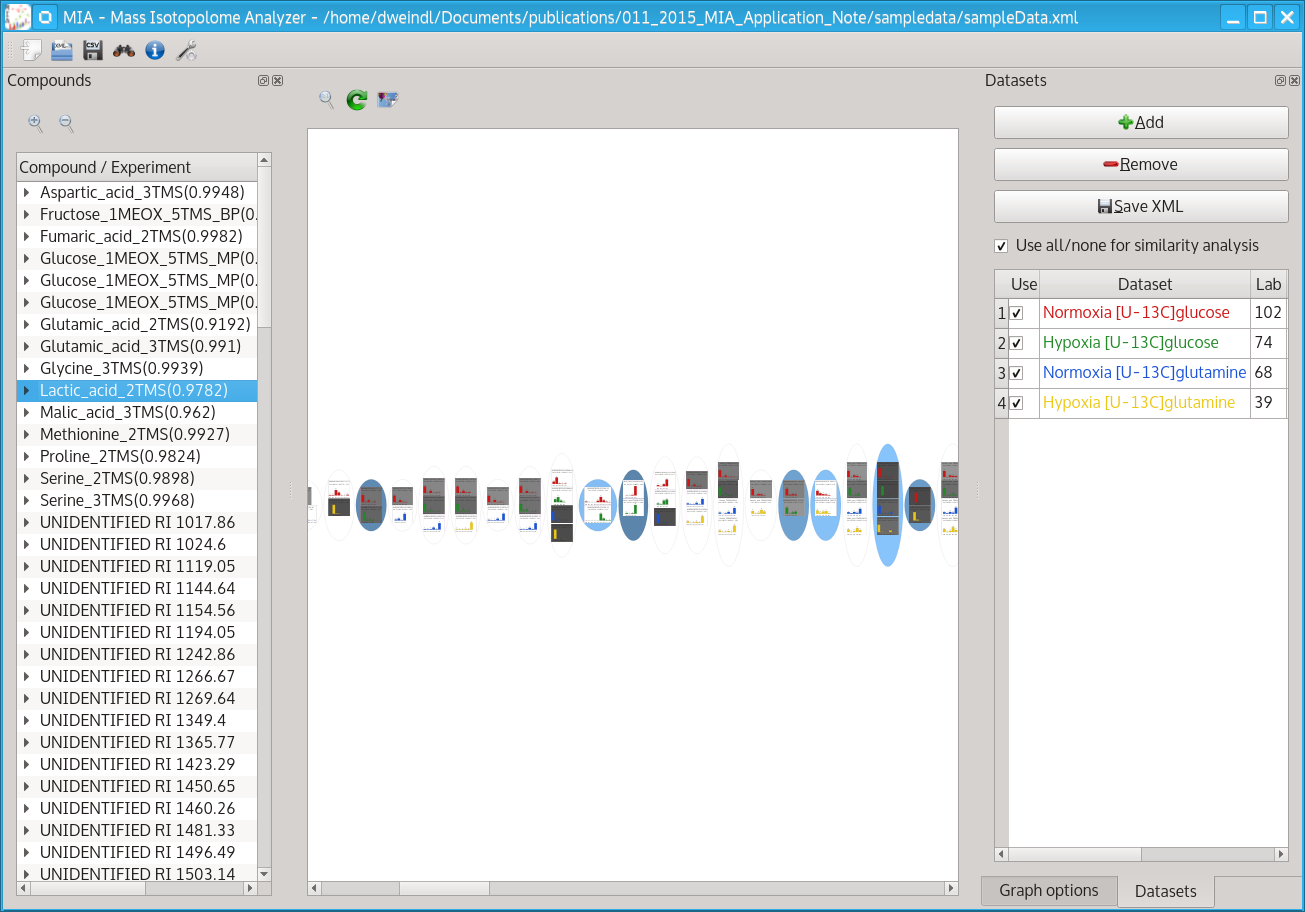
\includegraphics[width=0.8\textwidth]{./gfx/ss_tutorial_identified.png}
 \caption{\app\ after loading the sample dataset.}
 \label{fig:tutorial-identified}
\end{figure}

\subsubsection{MID variation}

You can use \app\ to detect those compounds with changing MIDs, which are indicative of changing fluxes in response to lower oxygen levels. To obtain meaningful results, only data from the same tracer should be used. Let's analyze isotopic enrichment from [U-$^{13}$C]glutamine. Therefor, first remove the [U-$^{13}$C]glucose labeling datasets by selecting them in the data set list and clicking ``remove''. For the MID variation analysis (\ref{sec:variation}), ideally the MIDs from the same mass spectrometric fragment is analyzed. To ensure this, access the configuration dialog from the main toolbar and select \textit{Misc} $\rightarrow$ \textit{Use largest common ion}.

%Now go to the ``Graph options'' tab, and set ``Minimum experiments for compounds'' to 2 and check ``Hide others''.

Check ``Hide others'' under ``Variation cutoff'' and move the slider slowly to the right. Some ellipses will start to disappear. Stop, when there are only 5 compounds left. Use the sample library as above to try to identify these compounds (Fig.~\ref{fig:tutorial-highvar}).

Malic acid and aspartic acid show a strong change in MIDs in response to lower oxygen availability. The strong increase in relative M+3 abundance and the strong decrease in M+4 abundance are indicative of an inversion of isocitrate dehydrogenase flux directionality, an important feature of cancer hypoxic cancer cells \citep{Wise2008,Metallo2012,Weindl2016}.

\begin{figure}[htbp]
 \centering
 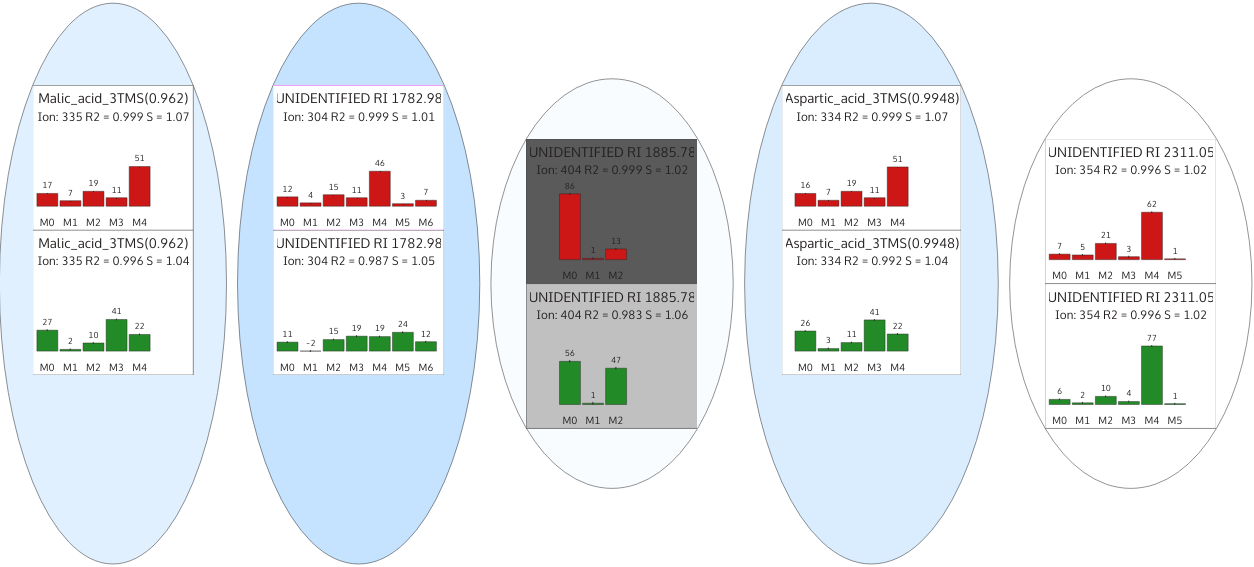
\includegraphics[width=0.8\textwidth]{./gfx/ss_tutorial_highvar.png}
 \caption{Hypoxia-induced changes after [U-$^{13}$C]glutamine labeling.}
 \label{fig:tutorial-highvar}
\end{figure}

\subsubsection{MID similarity}

Three other compounds of the five selected in the previous step are still unidentified. We try to gain information on their metabolic origin by comparing their MIDs to those of other compounds. Let's try that for the compound RI~1782.98.

In the configuration dialog, uncheck \textit{Misc} $\rightarrow$ \textit{Use largest common ion}. In the Graph options, uncheck ``Hide others'' under ``Variation cutoff'' and move slider back to 0. Now move the ``Distance cutoff'' slider slowly to the right, to about 1\%.
%In the warning dialog, click ``Yes'' if the edge number is still below 400, otherwise select a lower cutoff value.
When the graph is plotted, click on ``RI~1782.98'' in the compound list to center the view on it. The result will look similar to Fig.~\ref{fig:tutorial-midsim}.

\begin{figure}[htbp]
 \centering
 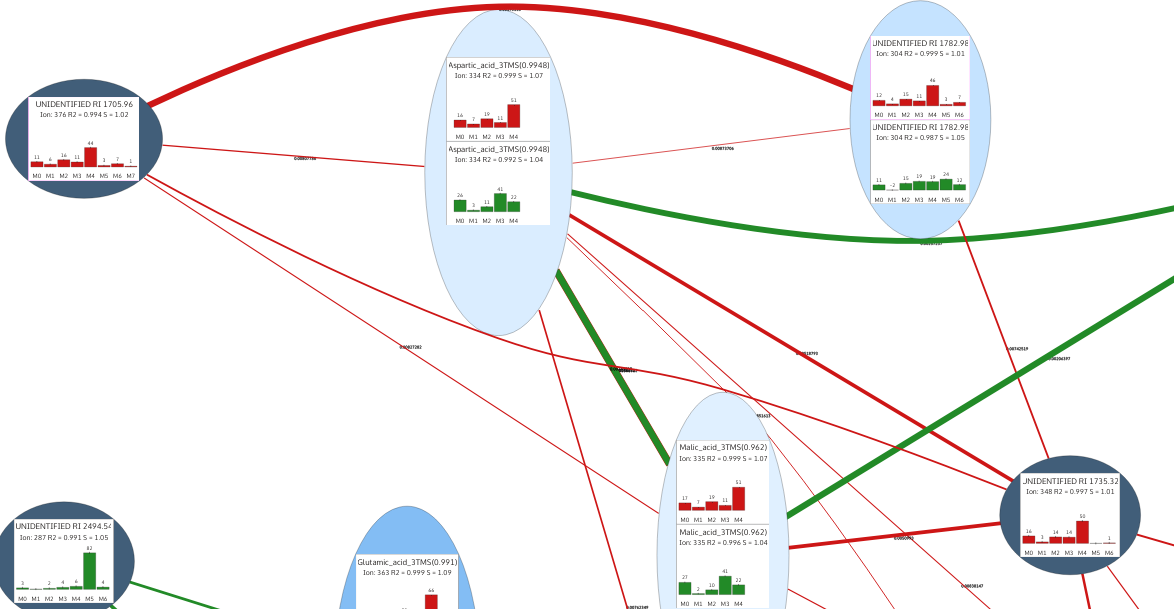
\includegraphics[width=0.8\textwidth]{./gfx/ss_tutorial_midsim.png}
 \caption{MID-neighbors of RI~1782.98.}
 \label{fig:tutorial-midsim}
\end{figure}

From the network you can see that our compound of interest RI~1782.98 is has a extremely similar MID as compound RI~1705.96. This is a hint, that both compounds are part of the same linear metabolic pathway, or that these are two derivatives arising during sample preparation from the same native metabolite.
Furthermore, aspartic acid and malic acid show high MID similarity at normoxia, and thus, seem to be closely related.

And indeed, a more comprehensive reference library will confirm these observations: RI~1782.98 and 1705.96 are the 3TMS and 2TMS derivative of \textit{N}-acetylaspartic acid, respectively. \textit{N}-acetylaspartic acid is derived from aspartic acid which is in turn derived from malic acid, explaining the high observed MID similarity.

%\subsubsection{Multiple datasets}

% load second data sets and introduce flux analysis

\subsubsection{Exporting the data}

Export the MIDs of all compound as csv file, by selecting 
\includegraphics{../gui/icons/document-save-csv.png} ``Export MIDs to CSV'' from the main toolbar. Export the MID plots currently shown in the graph view by selecting 
\includegraphics{gfx/ico_export-image.png} ``Export image'' in the graph view toolbar  (\ref{sec:graph-view}). Inspect the exported data in a spreadsheet application (.csv) and a vector graphics editor (.svg).

%\section{References}

\bibliographystyle{abbrv} 
\bibliography{mia-doc}
 
\end{document}
